\section{Sacred Science 103: The Vital Center}

\begin{figure}[t]
\centering
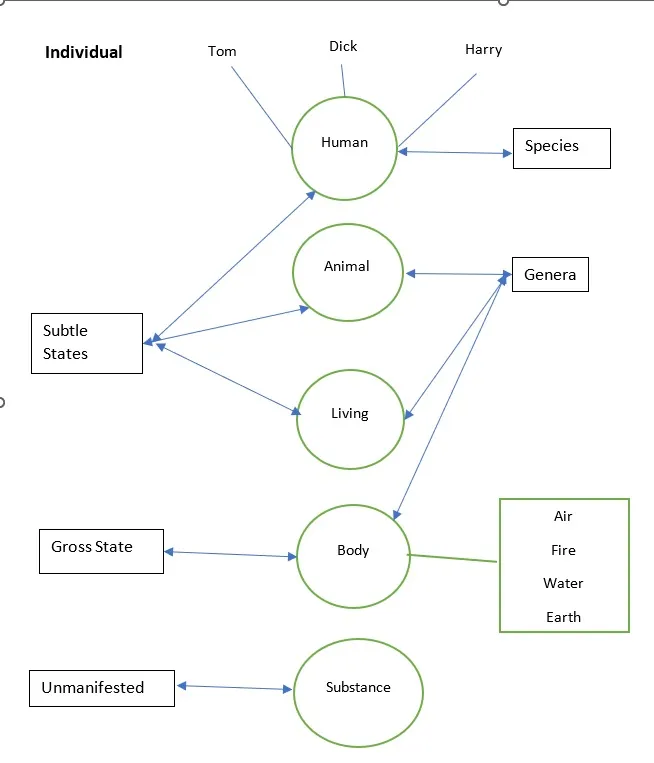
\includegraphics[scale=0.25]{a20220928SacredScience103TheVitalCenter-img001.png}
\caption{The manifestation of the Individuality}
\label{fig:SacredScience103_1}
\end{figure}
 
The diagram in Fig.~\ref{fig:SacredScience103_1} combines the two diagrams from the chapter, \emph{Self and Ego}, that illustrate the manifestation of the individuality. The unmanifested Primordial Substance potentially contains all the possibilities of manifestation. The gross state and the two subtle states are genera, and the human is the species. Particular individuals are manifestations of the species, although with special conditions that make each one unique.

The individual is not yet the Self or Atman, but as jivatman (living soul), it is the particular manifestation of the Self in life. The Atman is identical to Brahman. That identity is called the Supreme Identity, which must be realized (i.e., made real) through the intimate and essential union of the being with the Divine Principle.

\begin{wrapfigure}{rt}{0.3\textwidth}
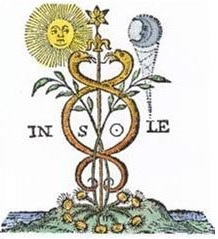
\includegraphics[scale=0.65]{a20220928SacredScience103TheVitalCenter-img002.jpg} 
\end{wrapfigure}
 
Nevertheless, Brahmin, or the Divine Spark, resides in the vital center of every human being, not just for the one who is united or liberated. The heart is the center of life and esoterically refers to the seat of intelligence and not of sentiment. The brain is only the instrument of the mental, i.e., of thought in a reflective and discursive mode. Symbolically, the heart corresponds to the sun and the brain to the moon.

The jivatman is like the image of the Atman, hence it is illusory in relationship to the Atman. The Self is only potentially in the individual, as long as the Union is not realized. However, the Self is not affected in any way by the realization.

\paragraph{Possibility and Potential}
Potential means the aptitude for a certain development and it supposes a possible actualization. It can be applied only in regard to becoming or manifestation. That is because the Self is complete in itself and has no unactualized potential.

But for the individual, all the possibilities that surpass him appear as potential as if he had his own being from himself. What he can attain is actually only a reflection, and not the possibilities themselves. Although this is only an illusion, one can say that these always remain potential for the individual, since he cannot attain them as an individual. As soon as all the possibilities are realized, there is truly no more individuality.


\bigskip

\flrightit{Posted on 2022-09-28 by Cologero}

\begin{center}* * *\end{center}

\begin{footnotesize}\begin{sffamily}

\texttt{Balder on 2022-10-05 at 09:14 said: }

“The two birds that reside in the same tree”, as the Mandokyua Upanishad puts it. I have lately thought about Odinn's ravens Hugin and Munin or the Eagle and the Hawk that reside in Yggdrasil; they might perform the same function of the Self and ego than in the Upanishadic Hindu tradition.

Although I personally see Hugin and Munin representing the left and the right hemispheres of the brain, who's to say they wouldn't have another function as well according to the traditional symbolism and the apparent duality of reason and logic \& imagination (“I Mage Nation”) and emotion. It is also integral to realize that in our bodily functions the left hemisphere guides the right hand and the right hemisphere the left hand.

It is not long ago that I read again Guénon's Man and His Becoming According to the Vedanta and Introduction to the Study of the Hindu Tradition, and there was a lot to ponder concerningthe Atma and jivatma and other correspondences. As I have been delving into the Nordic Traditions for the past 12 years, I have become to see Odinn and Wäinämöinen representing the Self and Loki and Joukahainen the ego, in hindu terms Odinn and Wäinämöinen is the Atman, Atma-Budhi, Christos etc. while other figures of mythology represent the different planetary powers (Thor / Jupiter, Odinn / Mercury, Freya / Venus, Tyr / Mars, Balder / Sun etc). Loki and Joukahainen are as the Norse equivalent of the male polarity of Lucifer or Satan, respectively.

\end{sffamily}\end{footnotesize}